\clearpage
\section{Architektura systemu deduplikacyjnego}
\label{sec:architektura-systemu}

Rozdział opisuje podział odpowiedzialności między komponentami,
przebieg deduplikacji oraz kolejność operacji na danych.
Przedstawiono stan implementacji, w tym ograniczenia jej spójności.
Sposób wyznaczania reprezentacji obrazów i oceny jakości omówiono
oddzielnie w podrozdziałach~\ref{sec:model-sscd}
i~\ref{sec:infogain-jakosc}; tutaj uwzględniono jedynie ich miejsce
w potoku.

\subsection{Założenia projektowe i wymagania}

Przy projektowaniu uwzględniono wolumen przechowywanych danych,
liczbę operacji na indeksach i koszt analizy obrazów.
Powiązanie decyzji technicznych z wykorzystaniem zasobów odpowiada
zasadom FinOps, w których optymalizację rozpatruje się w odniesieniu
do wartości dostarczanej przez system~\cite{finops_principles}.
Przyjęto następujące wymagania:

\begin{itemize}
    \item \textbf{Detekcja duplikatów binarnych:}
    rozpoznawanie identycznej zawartości przed analizą obrazu.
    \item \textbf{Detekcja kopii po przekształceniach:}
    porównywanie obrazów także po kompresji, skalowaniu lub innych
    modyfikacjach. Do takiego zadania opracowano reprezentację
    SSCD~\cite{pizzi2022sscd,sscd_repo}.
    \item \textbf{Wybór przechowywanej wersji:}
    umożliwienie podmiany podobnego obrazu na podstawie oceny jakości.
    \item \textbf{Ograniczona współbieżność:}
    kontrolowanie liczby jednocześnie przetwarzanych plików
    i buforowanych strumieni.
    \item \textbf{Kontrola spójności:}
    określenie zakresu ochrony przed współbieżnymi zapisami
    i skutków przerwania operacji obejmującej kilka magazynów.
\end{itemize}

Spełnienia wymagań wydajnościowych nie wywiedziono z samego doboru
technologii. Przepustowość, zużycie zasobów i efekty deduplikacji
podlegają pomiarom opisanym w rozdziale~\ref{chap:ewaluacja-i-finops}.

\subsection{Podział na komponenty i warstwę danych}
\label{subsec:architektura-hybrydowa}

System obejmuje dwa mikroserwisy połączone interfejsem gRPC.
W referencyjnej konfiguracji Docker Compose uruchamiane są one lokalnie,
razem z PostgreSQL i LocalStack. LocalStack udostępnia lokalną emulację
usług AWS, w tym S3 i DynamoDB, przeznaczoną do prac rozwojowych
i testów~\cite{localstack_overview}.
Konfiguracja ta nie stanowi wdrożenia usług w rzeczywistym środowisku AWS.

\begin{figure}[!h]
	\centering 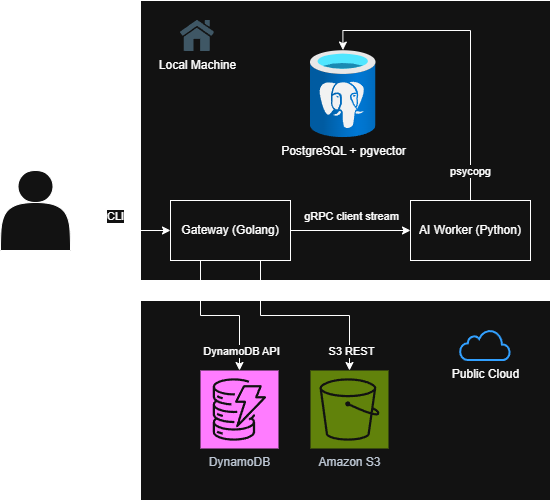
\includegraphics[width=0.5\linewidth]{HybridArchitectureDiagram.drawio.png}
	\caption{Architektura Hybrydowa}
\end{figure}

\begin{itemize}
    \item \textbf{Gateway w Go:}
    obsługuje CLI, odczyt plików, obliczanie skrótów i sterowanie
    potokiem. Wywołuje AI Workera oraz interfejsy S3 i DynamoDB.
    \item \textbf{AI Worker w Pythonie:}
    odbiera obrazy, dla których nie potwierdzono duplikatu binarnego.
    Wyznacza reprezentację i ocenę jakości, wyszukuje odpowiednik
    w PostgreSQL, a następnie zwraca wynik decyzji.
\end{itemize}

Warstwę danych podzielono według rodzaju informacji.
Interfejs S3 wykorzystano do zapisu obrazów i osobnych obiektów JSON,
DynamoDB do przechowywania metadanych plików i indeksu par skrótów, a PostgreSQL
z rozszerzeniem \texttt{pgvector} do przechowywania i przeszukiwania
reprezentacji wektorowych. Rozdzielenie tych zadań wykorzystuje
odpowiednio model obiektowy, odczyty według klucza i operacje
na wektorach~\cite{aws_s3_welcome_doc,awsGetItem,pgvector_docs}.
Wektory są zapisywane bezpośrednio przez AI Workera.
Nie są zwracane bramie.

Nazwę bazową pliku, uzyskaną przez \texttt{filepath.Base}, przyjęto
jako identyfikator aplikacyjny. Obraz zapisywany jest pod kluczem
\texttt{payloads/\allowbreak<file\_name>}, a jego opis pod
\texttt{metadata/\allowbreak<file\_name>.json}.
Opis JSON jest osobnym obiektem, nie zestawem metadanych użytkownika
dołączonych do obiektu obrazu.
W DynamoDB zastosowano dwa rodzaje rekordów:

\begin{itemize}
    \item \textbf{Rekord metadanych pliku:}
    \texttt{PK = FILE\#<file\_name>}, \texttt{SK = META};
    rekord zawiera m.in. klucz obiektu, rozmiar, wymiary i skróty.
    \item \textbf{Indeks zawartości:}
    \texttt{PK = CHUNK\#<c>}, \texttt{SK = FULL\#<h>};
    rekord wiąże skrót pierwszego fragmentu i całego pliku
    z zapisanym obiektem.
\end{itemize}

Osobno obsługiwane są powtarzające się nazwy bazowe w jednym
przetwarzanym zbiorze. Przed uruchomieniem zadań zachowywane jest
pierwsze wystąpienie, a następne zgłaszane są jako błędy wejścia.
Takie zachowanie wynika z przyjęcia nazwy bazowej jako identyfikatora,
również dla plików pochodzących z różnych katalogów.

\subsubsection{Dobór technologii: Go oraz Python}

Go wykorzystano do obsługi I/O i organizacji współbieżnego przetwarzania.
Goroutines są rozdzielane przez środowisko wykonawcze między wątki
systemowe; blokowanie podczas I/O nie musi zatrzymywać pozostałych
goroutines~\cite{go_effective}.
Mechanizm ten nie zastępuje synchronizacji współdzielonego stanu,
dlatego równoległość bramy ograniczono jawnie, jak opisano
w podrozdziale~\ref{subsec:wspolbieznosc}.

Python wykorzystano w części analitycznej z PyTorch.
Oficjalne repozytorium SSCD udostępnia modele TorchScript i przykłady
inferencji w tym środowisku~\cite{sscd_repo}.
Rozdzielenie usług pozwala zmieniać przygotowanie obrazu i inferencję
bez przenoszenia tej logiki do kodu obsługującego magazyny danych.
W badanej wersji model ładowany jest na CPU.

\subsubsection{Komunikacja za pomocą gRPC}
\label{subsubsec:grpc-komunikacja}

Kontrakt zdefiniowano w pliku \texttt{proto/dedup.proto}.
Na podstawie definicji usługi i wiadomości wygenerowano kod dla obu
języków, zgodnie z modelem pracy gRPC~\cite{grpc_core_concepts}.
Wykorzystany transport HTTP/2 obsługuje wiele strumieni w jednym
połączeniu; nie oznacza to jednak, że obiekt klienta musi utrzymywać
zawsze dokładnie jedno połączenie TCP~\cite{rfc9113,grpc_go_client}.

\begin{lstlisting}[
    language={},
    basicstyle=\ttfamily\small,
    numbers=left,
    firstnumber=1,
    breaklines=true,
    caption={Fragment kontraktu dedup.proto. Opracowanie własne.},
    label={lst:dedup-proto}
]
service ImageDedupService {
  rpc ProcessImageStream(stream ImageChunk)
      returns (ProcessImageResponse);
}

message ImageChunk {
  string image_key = 1;
  int64 total_size = 2;
  bytes data = 3;
  float threshold = 4;
}

message ProcessImageResponse {
  string status = 1;
  string image_key = 2;
  float quality_score = 3;
  float distance = 4;
  string existing_image_key = 5;
}
\end{lstlisting}

Metoda \texttt{ProcessImageStream} jest wywołaniem ze strumieniowaniem
po stronie klienta. Przesyłana jest sekwencja wiadomości
\texttt{ImageChunk}, po której odbierana jest pojedyncza odpowiedź;
gRPC zachowuje kolejność wiadomości w obrębie tego
wywołania~\cite{grpc_core_concepts}.
Pole \texttt{bytes} w Protocol Buffers przenosi dane binarne
z zakodowaną długością, bez konieczności zamiany obrazu
na tekst~\cite{protobuf_encoding}.

W bramie tworzony jest jeden współdzielony \texttt{grpc.ClientConn}.
Jest to kanał klienta, a nie zaimplementowana w aplikacji pula
połączeń~\cite{grpc_go_client}.
Adres określa zmienna
\texttt{AI\_\allowbreak WORKER\_\allowbreak GRPC\_\allowbreak ADDR},
domyślnie \texttt{localhost:50051}; w Docker Compose wskazano usługę
AI Workera. W tej konfiguracji nie zastosowano TLS ani osobnego
limitu czasu dla każdego RPC.
Brak jawnego terminu wywołania oznacza, że samo gRPC nie narzuca
takiego ograniczenia~\cite{grpc_deadlines}.

Stan transportu odróżniono od pola aplikacyjnego \texttt{status}.
Błędy RPC przekazywane są kodami gRPC, natomiast pole wiadomości
opisuje wynik deduplikacji~\cite{grpc_status_codes}.
AI Worker jawnie zwraca \texttt{INVALID\_ARGUMENT}, gdy nie otrzyma
klucza obrazu albo danych. Nie zaimplementowano pełnej walidacji
zadeklarowanego rozmiaru ani zakresu wartości progu.

\subsection{Logiczny potok deduplikacyjny}
\label{subsec:logiczny-potok}

Przed uruchomieniem potoku odczytywane są rozmiar pliku i konfiguracja
obrazu. Niepowodzenie dekodowania, w tym próba odczytu pustego pliku,
kończy przetwarzanie przed CDC i RPC.
W potoku zastosowano trzy etapy. Najpierw wykonywany jest
\texttt{ChunkPipeline}, następnie \texttt{FullHashPipeline},
a na końcu \texttt{SimilarityPipeline}.
Każdy zwraca decyzję \texttt{continue}, \texttt{accept\_full}
albo \texttt{soft\_dedup}. Pierwsza decyzja inna niż
\texttt{continue}, podobnie jak błąd, kończy wykonanie łańcucha.

Etapy jednego pliku wykonywane są sekwencyjnie; współbieżnie
przetwarzane są różne pliki.
Nie zbudowano oddzielnych procesów roboczych połączonych kanałami
dla każdego etapu. Jest to rozróżnienie względem potoków Go,
w których równoległe grupy goroutines przekazują dane przez
kanały~\cite{go_pipelines}.
Pominięcie dalszej analizy wynika z otrzymanej decyzji,
nie z założenia, że każdy kolejny etap musi trwać dłużej.

\subsubsection{Wstępne wyszukiwanie z wykorzystaniem CDC}
\label{subsubsec:potok-cdc}

Porcjowanie zależne od treści (ang. \textit{Content-Defined Chunking},
CDC) wyznacza granice fragmentów na podstawie danych, a nie wyłącznie
pozycji bajtów. Ogranicza przez to skutki przesunięcia granic po
wstawieniu lub usunięciu części zawartości, występujące w podziale
na bloki o stałej długości~\cite{gregoriadis2024cdc}.
W tym projekcie użyto tylko pierwszego fragmentu jako filtra
kandydatów. Nie zaimplementowano przechowywania i deduplikowania
wszystkich fragmentów pliku.

Zastosowano bibliotekę \texttt{restic/chunker} w wersji
\texttt{v0.5.0}, wykorzystującą kroczący odcisk
Rabina~\cite{restic2026chunker}.
Odcisk aktualizowany jest dla przesuwanego okna i służy do wyznaczenia
granicy, a nie do kryptograficznej identyfikacji
zawartości~\cite{gregoriadis2024cdc}.
W użytej wersji okno ma \(64\) bajty, a domyślny warunek podziału
sprawdza \(20\) najmłodszych bitów odcisku~\cite{restic2026code}.
W aplikacji ustawiono stały wielomian
\texttt{0x3DA3358B4DC173} stopnia \(53\).

Domyślne progi biblioteki wynoszą \(512\,\mathrm{KiB}\)
i \(8\,\mathrm{MiB}\), a parametr nominalnego średniego rozmiaru
odpowiada \(1\,\mathrm{MiB}\)~\cite{restic2026chunker,restic2026code}.
Dolny próg ogranicza poszukiwanie granicy, górny wymusza zakończenie
fragmentu; koniec pliku pozwala zwrócić również krótszy
fragment~\cite{restic2026code}.
Nominalny parametr nie gwarantuje takiej samej średniej w badanym
zbiorze danych~\cite{gregoriadis2024cdc}.

Implementacja przewiduje ponadto odczyt zastępczy.
Gdy sprawdzenie stopnia wielomianu nie przejdzie albo biblioteka
nie zwróci poprawnego, niepustego fragmentu, plik jest przewijany
do początku i odczytywane jest do \(64\,\mathrm{KiB}\).
Nie jest to wówczas podział CDC.
Bufor początkowy tej samej wielkości przekazywany do biblioteki
nie ogranicza prawidłowego fragmentu CDC do \(64\,\mathrm{KiB}\).

Niech \(C_1(f)\) oznacza fragment rzeczywiście zwrócony przez
\texttt{readFirstChunk}: pierwszy fragment CDC albo, w ścieżce
zastępczej, prefiks długości \(\min(|f|,64\,\mathrm{KiB})\).
Zdefiniowano dwa identyfikatory:

\begin{equation}
\label{eq:cdc-hashes}
c=\operatorname{SHA256}\!\left(C_1(f)\right),
\qquad
h=\operatorname{SHA256}(f).
\end{equation}

Definicję funkcji SHA-256 określa standard
FIPS~180-4~\cite{shs2015}.
Równanie~\eqref{eq:cdc-hashes} jest natomiast oznaczeniem przyjętym
w projekcie i nie zakłada jednoczesnego obliczenia obu skrótów.
W zwykłej ścieżce CDC plik krótszy niż \(512\,\mathrm{KiB}\)
stanowi cały pierwszy fragment; wtedy \(c=h\).
W ścieżce zastępczej taka równość wynika z objęcia całego pliku
prefiksem tylko dla rozmiaru nieprzekraczającego \(64\,\mathrm{KiB}\).

Po wyznaczeniu \(c\) wykonywana jest operacja \texttt{Query}
dla \texttt{PK = CHUNK\#<c>} z parametrem \texttt{Limit = 1}.
Limit ogranicza liczbę ocenianych elementów, nie stanowi ogólnej
gwarancji uzyskania jednego dopasowania po zastosowaniu
filtra~\cite{awsQuery}.
W badanym kodzie nie użyto \texttt{FilterExpression}, dlatego
obecność zwróconego elementu wystarcza do wskazania kandydata.
Wynik zapisywany jest we fladze \texttt{ChunkMatched}.

\begin{figure}[!htbp]
\centering
\begin{lstlisting}[
    language={},
    frame=single,
    basicstyle=\ttfamily\small,
    breaklines=true
]
c = sha256(readFirstChunk(file))
Query PK = CHUNK#c, Limit = 1
  miss -> skip exact full-hash lookup; similarity
  hit:
    h = sha256(file)
    GetItem PK = CHUNK#c, SK = FULL#h
      hit  -> binary soft-dedup
      miss -> similarity
\end{lstlisting}
\caption{Dwuetapowe wyszukiwanie duplikatu binarnego.
Opracowanie własne na podstawie implementacji.}
\label{fig:cdc-lookup-algo}
\end{figure}

\subsubsection{Weryfikacja pełnego skrótu i warunki kontynuacji}
\label{subsubsec:potok-full-hash}

Trafienie dla \(c\) nie potwierdza tożsamości plików.
Mogą one zawierać taki sam początkowy fragment i różnić się dalszą
zawartością. Nie jest to kolizja funkcji skrótu, ponieważ haszowany
fragment jest w obu przypadkach identyczny.
Po trafieniu plik otwierany jest ponownie, a \(h\) obliczane
z całej zawartości, łącznie z wcześniej odczytanym początkiem.

Następnie wykonywane jest \texttt{GetItem} dla
\texttt{PK = CHUNK\#<c>} i \texttt{SK = FULL\#<h>}.
Operacja odczytuje rekord po pełnym kluczu głównym, obejmującym
w tej tabeli klucz partycji i klucz sortowania~\cite{awsGetItem}.
Trafienie kończy łańcuch decyzją \texttt{soft\_dedup}.
Nie uruchamia się RPC ani zapisu kolejnej kopii obrazu.
Nadal zapisywany jest jednak obiekt JSON z metadanymi przetwarzania.

Niech \(\mathcal{I}\) oznacza ustalony zbiór par skrótów
\((c',h')\) w indeksie, a
\(\mathcal{C}=\{c'\mid \exists h':(c',h')\in\mathcal{I}\}\)
zbiór skrótów początkowych fragmentów.
Warunek rozpoznania duplikatu w gałęzi binarnej zapisano jako:

\begin{equation}
\label{eq:soft-dedup}
\operatorname{dup}_{\mathrm{bin}}(f)
\iff (c,h)\in\mathcal{I}.
\end{equation}

Jest to formalizacja schematu indeksowania, nie wzór zaczerpnięty
z definicji CDC. Obecność pary implikuje obecność \(c\)
w \(\mathcal{C}\), więc pierwsze zapytanie pozwala odroczyć
obliczenie \(h\), zamiast dostarczać osobnego kryterium tożsamości.
Predykatu \(\operatorname{dup}_{\mathrm{bin}}\) nie utożsamiono
z każdą decyzją \texttt{soft\_dedup}.
Dotyczy ona także statusu \texttt{duplicate\_rejected}
z gałęzi podobieństwa.
Zgodność skrótów przyjęto jako kryterium projektu, bez porównywania
plików bajt po bajcie i bez zakładania matematycznej niemożliwości
kolizji.

Jeżeli odczyty zakończą się poprawnie, kontynuacja do analizy
podobieństwa odpowiada warunkowi:

\begin{equation}
\label{eq:full-hash-continue}
\operatorname{continue}_{\mathrm{bin}}(f)
\iff
(c\notin\mathcal{C})
\;\lor\;
\bigl(c\in\mathcal{C}\land(c,h)\notin\mathcal{I}\bigr).
\end{equation}

W wykonaniu stosowana jest ocena warunkowa.
Brak kandydata pozwala przejść do analizy podobieństwa bez obliczania
\(h\) na potrzeby wyszukania duplikatu. Nie oznacza to pominięcia
pełnego skrótu przez cały proces: jeśli obraz zostanie zaakceptowany
do zapisu, brakujące \(h\) jest obliczane w \texttt{uploadImage}
przed przesłaniem danych i utworzeniem wpisu indeksu.

\begin{figure}[!htbp]
\centering
\begin{lstlisting}[
    language={},
    frame=single,
    basicstyle=\ttfamily\small,
    breaklines=true
]
no CHUNK#c:
  similarity without full hash in lookup stage
  accepted -> compute missing full hash before upload

CHUNK#c exists, no matching FULL#h:
  similarity with full hash already available
\end{lstlisting}
\caption{Dwie ścieżki kontynuacji po niepotwierdzeniu duplikatu.
Opracowanie własne na podstawie implementacji.}
\label{fig:full-hash-continue-algo}
\end{figure}

W kodzie nie ustawiono \texttt{ConsistentRead}.
W usłudze DynamoDB oznacza to domyślnie spójność ostateczną:
odczyt może nie uwzględniać niedawnego zapisu~\cite{aws_read_consistency}.
Równania~\eqref{eq:soft-dedup} i~\eqref{eq:full-hash-continue}
opisują regułę dla ustalonego stanu indeksu, nie atomowy obraz
dwóch kolejnych wywołań.
Brak trafienia oznacza zatem niepotwierdzenie duplikatu
w odczytanym stanie, a nie bezwarunkową gwarancję unikalności.

\subsection{Integracja z modułem analitycznym i obsługa wyników}
\label{subsec:similarity-grpc-pipeline}

\subsubsection{Przesłanie i buforowanie obrazu}

Po niepotwierdzeniu duplikatu binarnego plik otwierany jest ponownie
i przesyłany od początku metodą \texttt{ProcessImageStream}
usługi \texttt{dedup.v1.ImageDedupService}.
Podział transportowy jest niezależny od CDC.
W kliencie zastosowano bufor o pojemności
\(B=2\,\mathrm{MiB}=2\cdot2^{20}\) bajtów.
Każdy dodatni wynik wywołania \texttt{Read} wysyłany jest
w osobnej wiadomości.

Interfejs \texttt{io.Reader} dopuszcza odczyt krótszy od pojemności
bufora, także przed końcem danych~\cite{go_io_reader}.
Dla poprawnie przesłanego niepustego pliku, bez wcześniejszego
zakończenia strumienia, oznaczono przez \(b_i\) liczbę bajtów obrazu
w wiadomości \(i\), a przez \(s\) rozmiar pliku.
Wówczas:

\begin{equation}
\label{eq:message-count}
\sum_{i=1}^{n}b_i=s,\qquad
0<b_i\leq B
\quad\Longrightarrow\quad
n\geq\left\lceil\frac{s}{B}\right\rceil.
\end{equation}

Równość zachodzi, gdy wszystkie wiadomości poza ostatnią zawierają
pełne \(B\) bajtów danych. Nie jest to gwarancja obecnej implementacji,
ponieważ nie zastosowano dopełniania krótkich odczytów przez
\texttt{io.ReadFull}~\cite{go_io_reader}.
Równanie wynika z przyjętej pojemności bufora, a nie z właściwości
algorytmu CDC.

Pierwsza wiadomość zawiera dane obrazu oraz pola
\texttt{image\_key}, \texttt{total\_size} i \texttt{threshold}.
W kolejnych wiadomościach wypełniane jest tylko \texttt{data}.
Limit odbioru i wysyłania po stronie AI Workera ustawiono na
\(8\,\mathrm{MiB}\) na wiadomość.
Limit wiadomości gRPC nie ogranicza łącznego rozmiaru strumienia,
a do danych obrazu dochodzi narzut kodowania pól
Protocol Buffers~\cite{grpc_core_limits,protobuf_encoding}.

Po stronie odbiorcy użyto \texttt{SpooledTemporaryFile}
z progiem \(20\,\mathrm{MiB}\).
Po jego przekroczeniu bufor przechodzi z pamięci operacyjnej do pliku
tymczasowego~\cite{python_tempfile}.
AI Worker zbiera cały strumień, a dopiero potem uruchamia ocenę
jakości i inferencję. Strumieniowy transport nie oznacza więc
inferencji na niekompletnym obrazie.
Próg bufora nie jest też limitem całkowitej pamięci procesu,
ponieważ poza nim przechowywane są model i zdekodowane dane obrazu.

Jeżeli \texttt{Send} zwróci \texttt{io.EOF}, klient kończy wysyłanie
i wywołuje \texttt{CloseAndRecv}, aby odebrać wynik lub końcowy
status RPC. Jest to zgodne z możliwością zakończenia wywołania
przez serwer przed odebraniem wszystkich wiadomości
klienta~\cite{grpc_core_concepts}.
Inne błędy wysyłania przerywają przetwarzanie.

\subsubsection{Decyzja AI Workera}

Pole \texttt{threshold} przenosi maksymalną dopuszczalną odległość
kosinusową, domyślnie \(0{,}60\), a nie minimalne podobieństwo.
W zapytaniu do \texttt{pgvector} użyto operatora \texttt{<=>};
odpowiada on odległości kosinusowej, podczas gdy podobieństwo
wynosi jeden minus ta odległość~\cite{pgvector_docs}.
Definicję reprezentacji i dobór progu przedstawiono
w podrozdziałach~\ref{sec:reprezentacja-wektorowa}
i~\ref{sec:ewaluacja-progów}.

AI Worker wykonuje wyszukanie i ewentualną aktualizację
PostgreSQL przed zwróceniem odpowiedzi RPC.
Odpowiedź zawiera identyfikatory, ocenę jakości i odległość,
ale nie reprezentację wektorową.
W bramie status mapowany jest na dalsze działanie:

\begin{itemize}
    \item \textbf{\texttt{inserted}:}
    przyjmowany jest zapis obrazu.
    W PostgreSQL użyto operacji \texttt{INSERT ... ON CONFLICT},
    więc status nie gwarantuje utworzenia nowego wiersza przy
    ponownym użyciu tego samego \texttt{image\_key}.
    \item \textbf{\texttt{duplicate\_rejected}:}
    zwracana jest decyzja \texttt{soft\_dedup}.
    Pomijany jest zapis obrazu i wpisów DynamoDB, ale zapisywany
    jest obiekt JSON.
    \item \textbf{\texttt{replaced}:}
    przyjmowany jest zapis obrazu i ustawiana flaga
    \texttt{ReplaceExisting}. Rekord PostgreSQL aktualizowany
    jest w miejscu przez \texttt{UPDATE}, bez poprzedzającego
    \texttt{DELETE}.
\end{itemize}

\subsubsection{Kolejność zapisu i wycofanie poprzedniej wersji}

Po poprawnym zakończeniu łańcucha serializowany i zapisywany jest JSON.
Przy \texttt{soft\_dedup} proces kończy się na tym etapie.
Dla zaakceptowanego obrazu najpierw uzupełniany jest brakujący pełny
skrót. Następnie obraz zapisywany jest pod kluczem
\texttt{payloads/\allowbreak<file\_name>}.
Na końcu zapisywane są rekord metadanych pliku
\texttt{FILE\#\allowbreak<file\_name>/\allowbreak META}
i para \texttt{CHUNK\#<c>/\allowbreak FULL\#<h>}.
Są to oddzielne operacje, a nie jedna transakcja.

Funkcja \texttt{retireReplaced} uruchamiana jest dopiero po
poprawnym zapisaniu nowego obrazu i obu wpisów indeksu.
Jeżeli \texttt{existing\_image\_key} różni się od nowej nazwy,
odczytywany jest stary rekord metadanych pliku, a następnie usuwane są:
poprzedni obraz, jego JSON, rekord metadanych oraz, jeśli odczytano
potrzebne skróty, rekord zawartości.
Przy identycznym kluczu osobne usuwanie jest pomijane.
Żadna z tych ścieżek nie usuwa lokalnego pliku źródłowego.

Skrypt inicjalizacyjny nie włącza wersjonowania zasobnika.
Nie należy jednak utożsamiać tego z gwarancją konfiguracji każdego
środowiska, do którego zostanie podłączona brama.
Przy włączonym wersjonowaniu S3 ponowny zapis pod tym samym kluczem
tworzy nową wersję, a usunięcie bez identyfikatora wersji dodaje
znacznik usunięcia zamiast kasować wcześniejsze
wersje~\cite{aws_s3_versioning_workflows}.

Dla statusu \texttt{replaced} rozmiar poprzedniego obrazu
odczytywany jest przez \texttt{HeadObject}.
Niech \(k_{\mathrm{old}}\) i \(k_{\mathrm{new}}\) oznaczają klucze,
a \(s_{\mathrm{old}}\) i \(s_{\mathrm{new}}\) rozmiary w bajtach.
Licznik projektu ma postać:

\begin{equation}
\label{eq:deleted-bytes}
\texttt{deleted\_bytes}=
\begin{cases}
0, & \text{gdy odczyt rozmiaru nie powiedzie się},\\
\max(0,s_{\mathrm{old}}-s_{\mathrm{new}}),
    & \text{gdy }k_{\mathrm{old}}=k_{\mathrm{new}},\\
s_{\mathrm{old}},
    & \text{gdy }k_{\mathrm{old}}\neq k_{\mathrm{new}}.
\end{cases}
\end{equation}

Dwie ostatnie gałęzie zakładają poprawny odczyt rozmiaru.
Przy tym samym kluczu liczona jest dodatnia różnica rozmiarów,
przy różnych kluczach cały rozmiar poprzedniego obiektu.
Nie jest to zatem jednolita miara oszczędności netto.
Ponadto S3 rozlicza zachowane wersje jako pełne obiekty,
nie różnice między wersjami~\cite{aws_s3_versioning_workflows}.
Interpretację kosztową pozostawiono analizie
w rozdziale~\ref{chap:ewaluacja-i-finops}.

\subsection{Miejsce oceny jakości w potoku}
\label{subsec:logika-decyzyjna}

Ocenę podobieństwa oddzielono od wyboru przechowywanej wersji.
Pierwsza wskazuje kandydata, druga rozstrzyga decyzję obsługiwaną
przez AI Workera. W bramie nie występuje osobny etap
\texttt{InfoGain}; klasa \texttt{SimilarityPipeline} odbiera
gotowy status i ustawia decyzję zapisu.
Plik \texttt{decision.go} definiuje możliwe decyzje potoku,
nie algorytm oceny jakości.

Wynik oceny przekazywany jest w polu \texttt{quality\_score}.
Pole \texttt{existing\_image\_key} wskazuje obiekt podlegający
ewentualnemu wycofaniu.
Definicję wskaźnika, kierunek porównania i obsługę remisu przedstawiono
w podrozdziale~\ref{sec:infogain-jakosc}.

\subsection{Współbieżność i zakres gwarancji spójności}
\label{subsec:wspolbieznosc}

\subsubsection{Limity i anulowanie pracy}

Do ograniczenia współbieżności użyto pakietu \texttt{errgroup}.
Grupę tworzono przez \texttt{WithContext}, a limit ustawiano
metodą \texttt{SetLimit}.
Parametr \texttt{--workers} ma domyślną wartość \(10\);
przyjęto co najmniej jedno zadanie.
\texttt{SetLimit} ogranicza liczbę aktywnych goroutines grupy,
a dodanie następnej może oczekiwać na zwolnienie
miejsca~\cite{go_errgroup}.
Nie jest to stała pula połączona kolejką aplikacyjną.

Wewnętrznie \texttt{errgroup} może anulować kontekst po zwróceniu
pierwszego błędu przez zadanie~\cite{go_errgroup}.
W tej aplikacji błędy pojedynczych obrazów są jednak rejestrowane,
a funkcja zadania zwraca \texttt{nil}.
Niepowodzenie jednego pliku nie przerywa więc automatycznie całego
zbioru; po zakończeniu zliczane są nieudane operacje.
Kontekst obsługuje natomiast przerwanie przez \texttt{SIGINT}
lub \texttt{SIGTERM}.

AI Worker wykorzystuje \texttt{ThreadPoolExecutor} z limitem
czterech wątków obsługi gRPC.
Przed rozpoczęciem przyjmowania wywołań inicjalizowany jest schemat
bazy i ładowany model.
Limit ten jest niezależny od liczby zadań bramy i nie stanowi
gwarancji czterokrotnego przyspieszenia inferencji.
Próg buforowania \(20\,\mathrm{MiB}\) dotyczy pojedynczego
strumienia, nie sumy danych wszystkich żądań.

\subsubsection{Transakcja decyzji i operacje między magazynami}

W \texttt{Repository.resolve} otwierana jest transakcja PostgreSQL.
Następnie pobierana jest blokada
\texttt{pg\_\allowbreak advisory\_\allowbreak xact\_\allowbreak lock}
ze stałym identyfikatorem \(74821001\).
Transakcyjne blokady doradcze są zwalniane na końcu transakcji
i wymagają współpracy aplikacji używających tej samej
konwencji~\cite{postgres16_locking}.
Wspólny identyfikator szereguje całe sekcje rozstrzygania decyzji
w tej samej bazie, również dla różnych obrazów.
Blokada nie obejmuje wcześniejszego obliczania reprezentacji
i jakości.

Przy odczycie jakości istniejącego obrazu stosowane jest także
\texttt{SELECT ... FOR UPDATE}.
Taka blokada chroni wskazany wiersz przed konkurencyjną modyfikacją
do końca transakcji~\cite{postgres16_locking}.
Wyjście z kontekstu transakcji Psycopg kończy się zatwierdzeniem
albo wycofaniem zmian zależnie od wystąpienia
wyjątku~\cite{psycopg_transactions}.
Zatwierdzenie następuje przed zwróceniem odpowiedzi do bramy.

Ochrona PostgreSQL nie obejmuje późniejszych zapisów JSON, obrazu
i indeksów DynamoDB. W kodzie nie zastosowano wspólnej transakcji,
zapisów warunkowych DynamoDB ani procedury kompensacji po błędzie.
Przerwanie po aktualizacji PostgreSQL może zatem pozostawić
rekord wektorowy bez odpowiadającego mu nowego obrazu;
przerwanie kolejnych zapisów może pozostawić niepełny indeks.
Nie można na tej podstawie zadeklarować atomowej podmiany
we wszystkich magazynach.

Pozostaje też ograniczenie podmiany pod tą samą nazwą.
\texttt{retireReplaced} pomija wtedy czyszczenie, mimo że nowy zapis
może dotyczyć innych skrótów. Stary rekord
\texttt{CHUNK\#<c>/\allowbreak FULL\#<h>} może nadal wskazywać nadpisany obiekt.
Z tego względu poprawność kolejnego trafienia binarnego zależy
również od aktualności indeksu, a nie wyłącznie od zgodności
skrótów. Ograniczenie to wymaga usunięcia w implementacji
lub uwzględnienia w ocenie wyników.

% \subsection{Perspektywa docelowa: wdrożenie chmurowe w AWS}
% \label{subsec:architektura-cloud-native}

% Przeniesienie analizy z urządzenia klienta do AWS stanowi wariant
% rozwojowy. Poniżej przedstawiono jego założenia i ograniczenia,
% nie wyniki wdrożenia. Wariant z instancjami EC2 nie jest traktowany
% jako rozwiązanie w całości bezserwerowe.

% \subsubsection{Model operacyjny i punkt wejścia CLI}
% \label{subsubsec:cloud-cli}

% CLI może pozostać punktem wejścia uruchamianym lokalnie, natomiast
% analiza obrazu może zostać przeniesiona do usług chmurowych.
% Wymaga to ustalenia miejsca deduplikacji względem pierwszego zapisu.
% Jeżeli analiza jest uruchamiana dopiero po zapisaniu obiektu
% w S3, nie eliminuje tego początkowego transferu ani operacji zapisu.
% Nie jest więc funkcjonalnie równoważna obecnemu filtrowaniu
% przed wysłaniem pliku do magazynu.
% % TODO[ARCH-14]: Wybrać wariant: analiza przed zapisem docelowym
% % albo zapis w obszarze tymczasowym i późniejsze przetwarzanie.

% \subsubsection{Asynchroniczne przetwarzanie z wykorzystaniem Amazon SQS}
% \label{subsubsec:cloud-sqs}

% W wariancie po zapisie można wykorzystać powiadomienia o utworzeniu
% obiektu S3 kierowane do kolejki Amazon SQS~\cite{aws_s3_events}.
% Kolejka standardowa dostarcza wiadomości co najmniej raz
% i może zmienić ich kolejność~\cite{aws_sqs_standard}.
% Projekt konsumenta musi zatem uwzględniać ponowne otrzymanie zdarzenia
% oraz zdarzenia dotyczące różnych wersji obiektu.
% Zastąpienie synchronicznego RPC takim przepływem wymaga również
% określenia sposobu odbioru wyniku przez CLI.
% % TODO[ARCH-15]: Określić identyfikację zadania, idempotencję,
% % ponowienia, obsługę błędów i sposób raportowania wyniku użytkownikowi.

% \subsubsection{Warstwa obliczeniowa AI: AWS Lambda lub EC2 z GPU}
% \label{subsubsec:cloud-ai-compute}

% Do dalszej oceny przewidziano AWS Lambda i instancje EC2 z GPU.
% Dobór wariantu Lambda wymaga sprawdzenia limitów czasu wykonania
% i pamięci w danym trybie usługi~\cite{aws_lambda_quotas}.
% AWS udostępnia także instancje EC2 z akceleratorami GPU,
% które mogą stanowić środowisko obliczeniowe modułu
% analitycznego~\cite{aws_ec2_accelerated}.
% Wybór powinien wynikać z pomiarów czasu inicjalizacji modelu,
% inferencji i wykorzystania zasobów, a nie z samej nazwy usługi.
% % TODO[ARCH-16]: Zmierzyć cold start, przepustowość i koszt.
% % Uzasadnienie wyboru wobec Amazon Bedrock pozostawić do czasu
% % określenia konkretnej usługi, modelu i wymagań inferencji.

% \subsubsection{Warstwa danych: DynamoDB i Aurora PostgreSQL}
% \label{subsubsec:cloud-data-layer}

% Wariant chmurowy może zachować S3 jako magazyn obiektów
% i DynamoDB jako indeks skrótów.
% Aurora PostgreSQL obsługuje rozszerzenie \texttt{pgvector}
% oraz wyszukiwanie wektorowe w wariancie Serverless
% v2~\cite{aws_aurora_vectors}.
% Samo przeniesienie bazy nie rozstrzyga jednak wyboru indeksu
% wektorowego: \texttt{pgvector} oferuje wyszukiwanie dokładne
% oraz indeksy przybliżone HNSW i IVFFlat~\cite{pgvector_docs}.
% Konfiguracja docelowa wymaga więc osobnej oceny jakości wyszukiwania,
% opóźnienia i kosztu.
% % TODO[ARCH-17]: Ustalić wersję silnika i rozszerzenia, typ indeksu,
% % konfigurację połączeń oraz parametry skalowania.
